\documentclass{beamer}

\mode<presentation>
{
  \usetheme{Boadilla}
  \usecolortheme{dove}
  \setbeamertemplate{page number in head/foot}{}
}

\usepackage[english]{babel}
\usepackage[utf8]{inputenc}
\usepackage{times}
\usepackage[T1]{fontenc}
\usepackage{graphicx}
\usepackage[normalem]{ulem}
\usepackage{array}
\graphicspath{ {images/} }

\definecolor{codegray}{gray}{0.9}
\newcommand{\code}[1]{{\texttt{#1}}}
%\colorbox{codegray}

\title[]
{\Huge{Komunikacja komponentów w aplikacji webowej}}

\author[Adrian Mularczyk]{\Large{Adrian Mularczyk}}

\institute[PGS Software]
{
\small{PGS Software}
}

\date{}

\begin{document}

\begin{frame}
  \titlepage 
\end{frame}

\begin{frame}{}
	\begin{tabular}{ p{4.4cm} p{6cm} }
		\begin{minipage}{.4\textwidth}
			\begin{center}
  				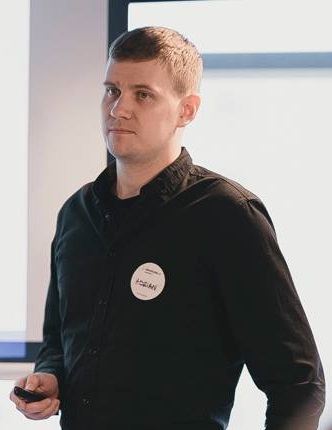
\includegraphics[height=5cm]{ja.jpg}
			\end{center}
   		 \end{minipage}
   		 &
		\begin{minipage}{.7\textwidth}
  					\Huge{Adrian Mularczyk} \newline \newline
					\Large{7 lat doświadczenia} \newline
					\Large{praca od 3 rok studiów}\newline
					\Large{Uniwersytet Wrocławski}
   		 \end{minipage}
	\end{tabular}
\end{frame}

\begin{frame}{}
	\begin{center}
		\Huge{Tak to się zaczęło...}
	\end{center}
\end{frame}

\begin{frame}{}
	\begin{center}
  		
\includegraphics[height=4cm]{lunch1.png}
	\end{center}
\end{frame}

\begin{frame}{}
	\begin{center}
		\Huge{Aplikacja webowa}
	\end{center}
\end{frame}

\begin{frame}{Aplikacja webowa}
	\begin{huge}
		\begin{itemize}[<+->]
			\item Aplikacja Mobilna
			\item Single Sing-On (SSO)
		\end{itemize}
	\end{huge}
\end{frame}

\begin{frame}{}
	\begin{center}
		\Huge{Single Sing-On (SSO)}
	\end{center}
\end{frame}

\begin{frame}{SSO}
	\begin{center}
  		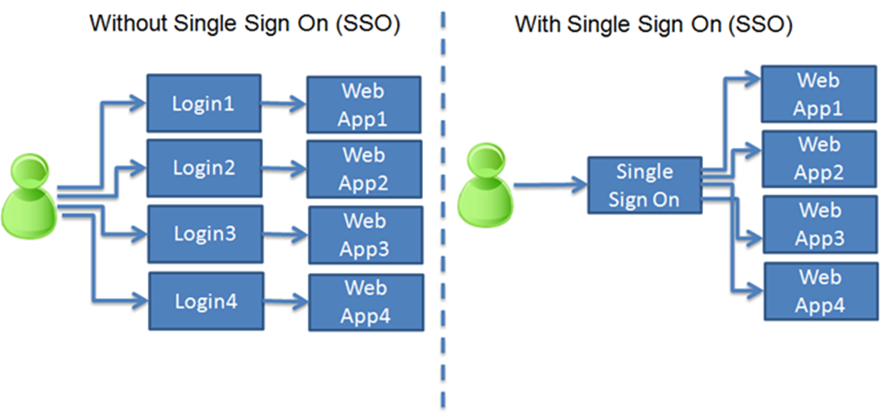
\includegraphics[height=5cm]{sso2.png}
	\end{center}
\end{frame}

\begin{frame}{Aplikacja webowa}
	\begin{huge}
		\begin{itemize}
			\item Frontend
			\item Backend (API)
			\item Identity (Autentykacja)
		\end{itemize}
	\end{huge}
\end{frame}

\begin{frame}{Aplikacja webowa}
	\begin{center}
		\Huge{Wspólny code -> Core}
	\end{center}
\end{frame}

\begin{frame}{}
	\begin{center}
		\Huge{Nuget}
	\end{center}
\end{frame}

\begin{frame}{Nuget}
	\begin{center}
  		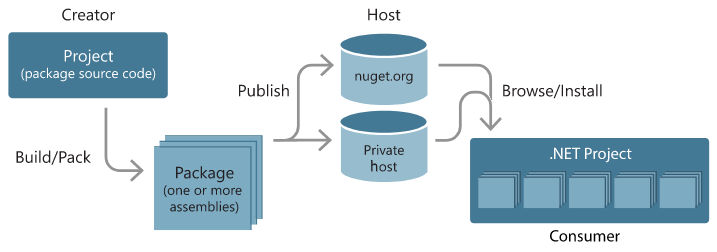
\includegraphics[height=4cm]{nuget1.png}
	\end{center}
\end{frame}

\begin{frame}{Nuget}
	\begin{center}
  		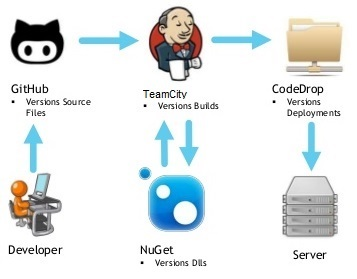
\includegraphics[height=5cm]{nuget2.jpg}
	\end{center}
\end{frame}

\begin{frame}{Aplikacja webowa}
	\begin{center}
		\begin{tabular}{ m{5cm} m{5cm} }
  			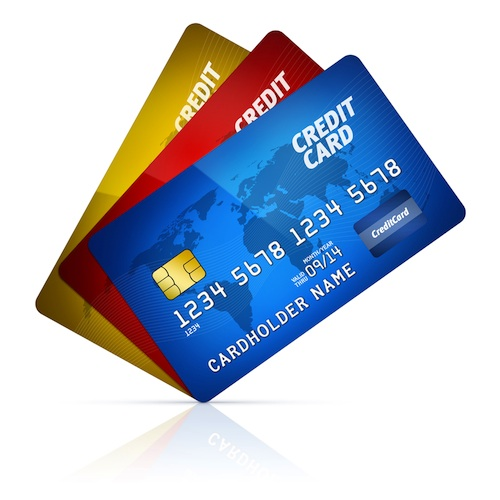
\includegraphics[height=3cm]{card3.jpg} & 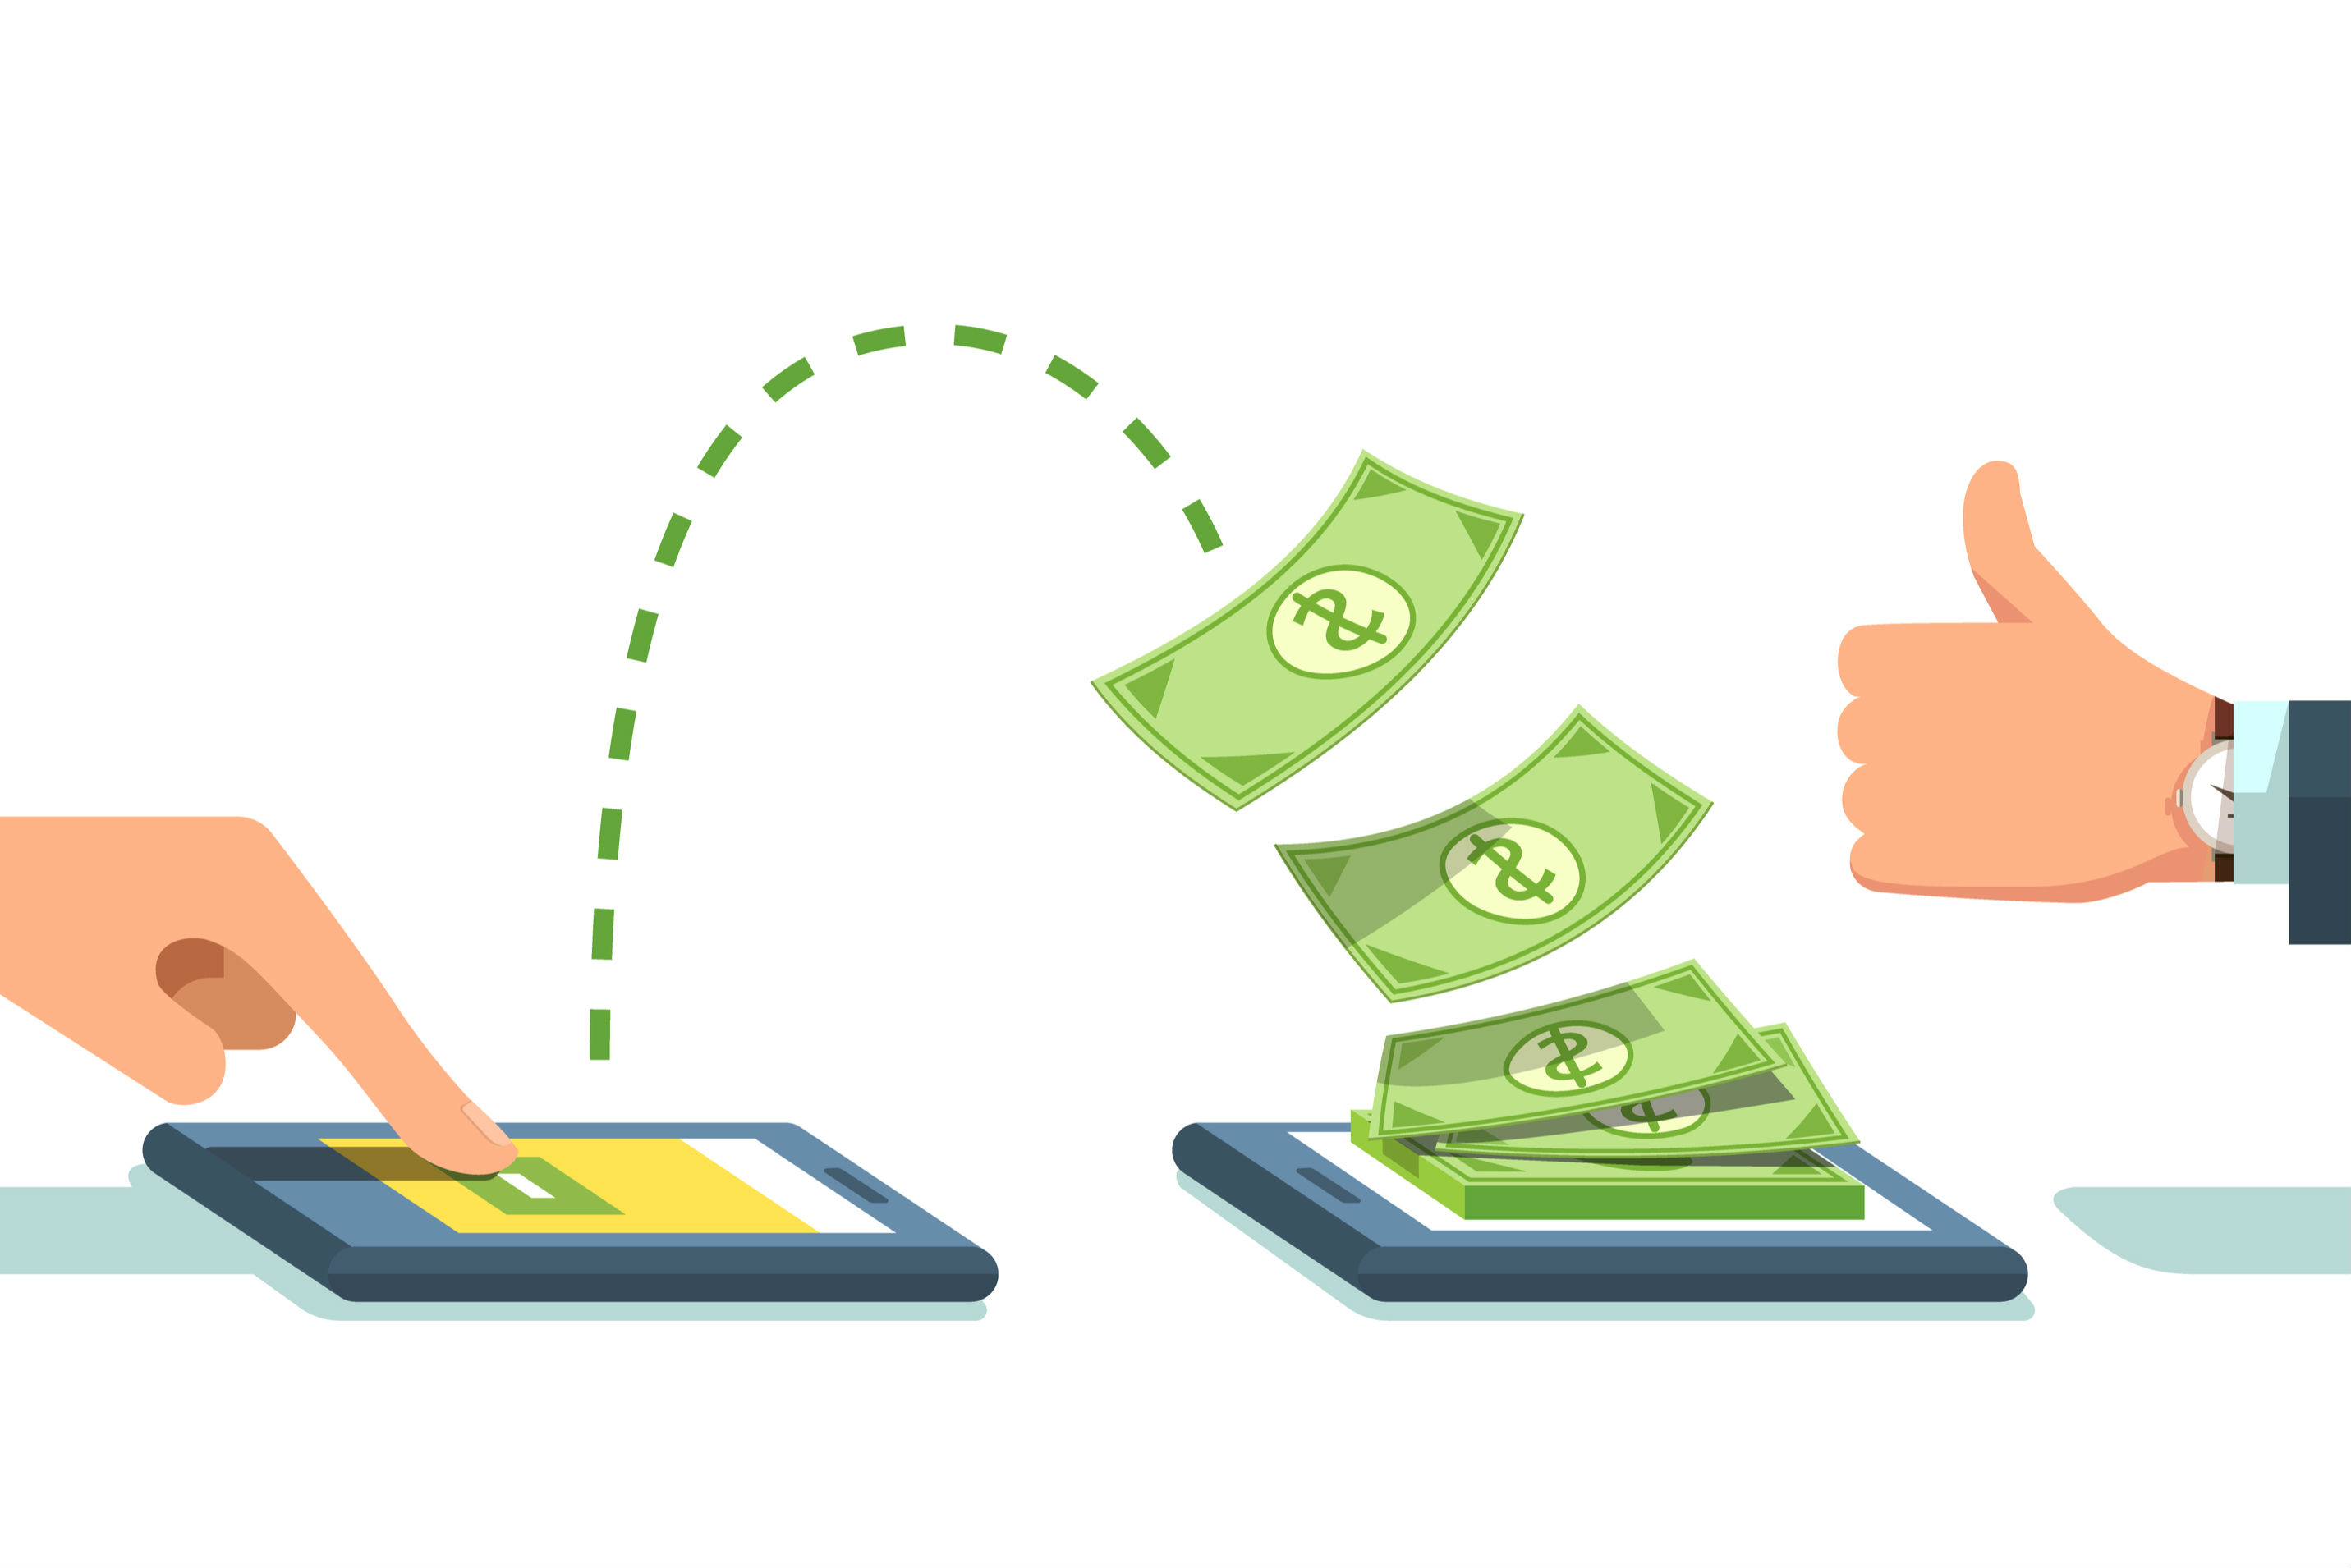
\includegraphics[height=3cm]{przelew1.jpg}
		\end{tabular}
	\end{center}
\end{frame}

\begin{frame}{Płatność kartą}
	\begin{center}
  		
\includegraphics[height=3cm]{request4.png}
	\end{center}
\end{frame}

\begin{frame}{Płatność kartą}
	\begin{center}
		
\includegraphics[height=3cm]{response1.png}
	\end{center}
\end{frame}

\begin{frame}{Płatność kartą - status}
	\begin{huge}
		\begin{itemize}[<+->]
			\item Accepted
			\item Failed
			\item Pending
		\end{itemize}
	\end{huge}
\end{frame}

\begin{frame}{Płatność kartą - Pending}
	\begin{center}
		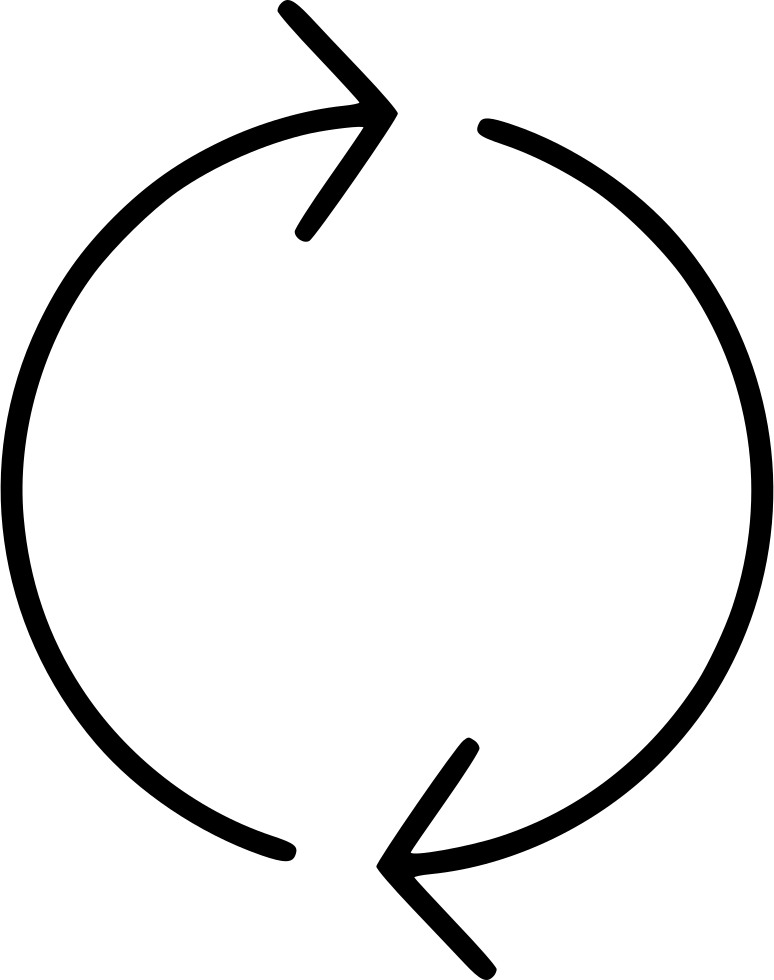
\includegraphics[height=4cm]{cykl1.png}
	\end{center}
\end{frame}

\begin{frame}{Płatność przelewem}
	\begin{huge}
		\begin{itemize}[<+->]
			\item Faktura
			\item Integracja z systemem zewnętrznym
		\end{itemize}
	\end{huge}
\end{frame}

\begin{frame}{Aplikacja webowa}
	\begin{center}
		\Huge{<<rozszerzyc>>}
	\end{center}
\end{frame}

\begin{frame}{Komunikacja komponentów}
	\begin{center}
		\Huge{Komunikacja synchroniczna}
	\end{center}
\end{frame}

\begin{frame}{Komunikacja synchroniczna}
	\begin{center}
		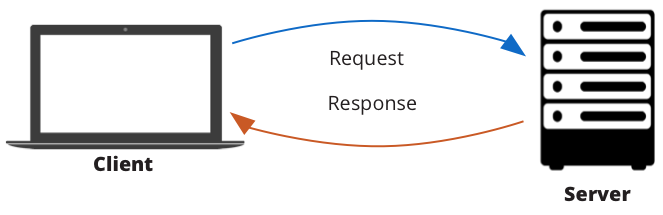
\includegraphics[height=3cm]{prosta_komunikacja2.png}
	\end{center}
\end{frame}

\begin{frame}{Aplikacja webowa}
	\begin{center}
		\Huge{Problemy}
	\end{center}
\end{frame}

\begin{frame}{Aplikacja webowa}
	\begin{center}
		\Huge{<<rozszerzyc>>}
	\end{center}
\end{frame}

\begin{frame}{}
	\begin{center}
		\Huge{Klient miał kolejne plany...}
	\end{center}
\end{frame}

\begin{frame}{}
	\begin{center}
		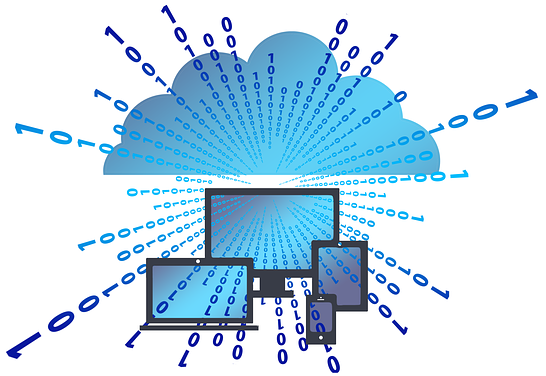
\includegraphics[height=4cm]{virtual1.png}
	\end{center}
\end{frame}

\begin{frame}{Nowe aplikacje}
	\begin{huge}
		\begin{itemize}[<+->]
			\item Pracownik
			\item Restauracja
		\end{itemize}
	\end{huge}
\end{frame}

\begin{frame}{Nowe aplikacje}
	\begin{huge}
		\begin{itemize}
			\item Frontend
			\item Backend (API)
			\item Identity (Autentykacja)
		\end{itemize}
	\end{huge}
\end{frame}

\begin{frame}{Nowe aplikacje}
	\begin{huge}
		\begin{itemize}[<+->]
			\item Identity
			\item Core
			\item Common
		\end{itemize}
	\end{huge}
\end{frame}

\begin{frame}{Architektura}
	\begin{center}
		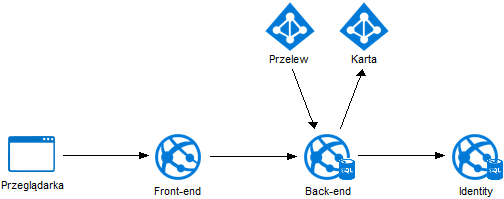
\includegraphics[height=4cm]{architektura1.png}
	\end{center}
\end{frame}

\begin{frame}{Architektura}
	\begin{center}
		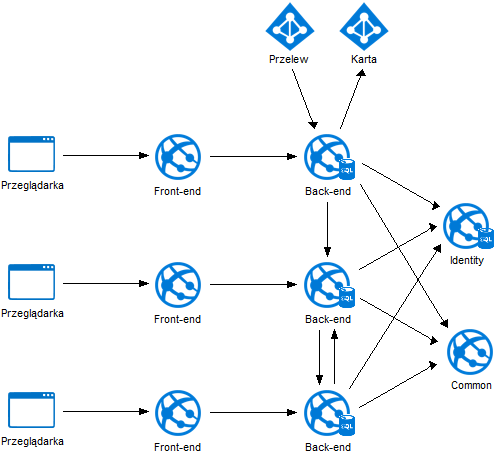
\includegraphics[height=7cm]{architektura2.png}
	\end{center}
\end{frame}

\begin{frame}{Architektura}
	\begin{center}
		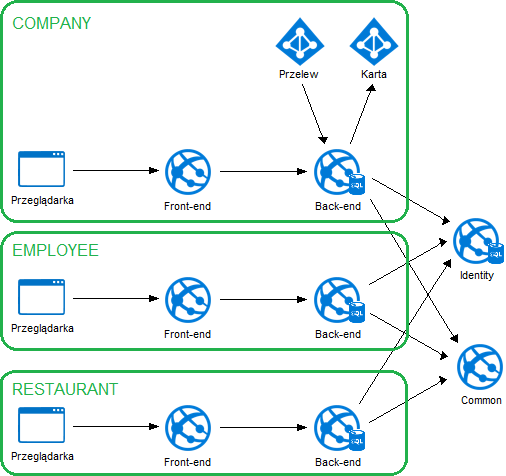
\includegraphics[height=8cm]{architektura4.png}
	\end{center}
\end{frame}

\begin{frame}{Komunikacja}
	\begin{huge}
		\begin{itemize}[<+->]
			\item Company -> Employee
			\item Employee -> Restaurant
			\item Restaurant -> Employee
		\end{itemize}
	\end{huge}
\end{frame}

\begin{frame}{Architektura}
	\begin{center}
		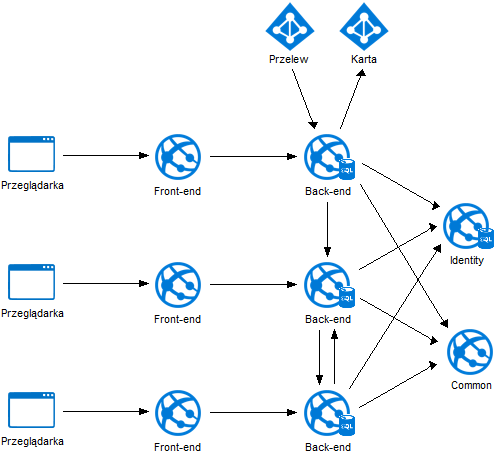
\includegraphics[height=8cm]{architektura3.png}
	\end{center}
\end{frame}

\begin{frame}{Nowe aplikacje}
	\begin{center}
		\Huge{Problemy}
	\end{center}
\end{frame}

\begin{frame}{Problemy}
	\begin{center}
		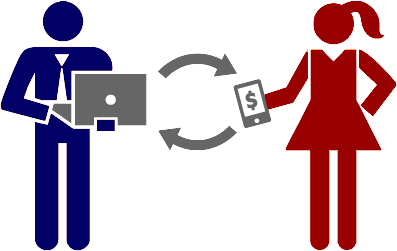
\includegraphics[height=4cm]{pay1.png}
	\end{center}
\end{frame}

\begin{frame}{Komunikacja komponentów}
	\begin{center}
		\Huge{Fire-and-forget}\\
		\huge{(komunikacja asynchroniczna)}
	\end{center}
\end{frame}

\begin{frame}{Fire-and-forget}
	\begin{center}
		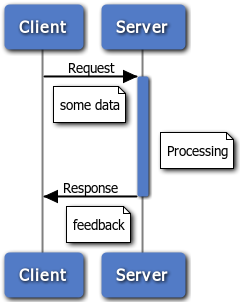
\includegraphics[height=4cm]{async1.png}
	\end{center}
\end{frame}

\begin{frame}{Fire-and-forget}
	\begin{center}
		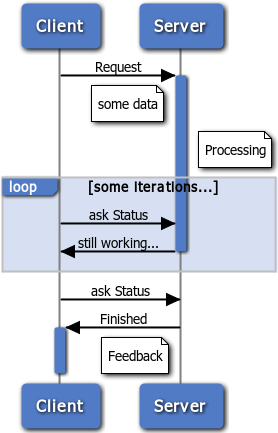
\includegraphics[height=6cm]{async2.png}
	\end{center}
\end{frame}

\begin{frame}{Problemy}
	\begin{Large}
		\begin{itemize}[<+->]
			\item 1. Pracownik płaci za lunch
			\item 2. Pracownik oczekuje na akceptację
			\item 3. Restauracja akceptuje płatność - 30 sekund
			\item 4. Restauracja powiadamia Pracownika
			\item 5. Aktualizacja statusu zamówienia
		\end{itemize}
	\end{Large}
\end{frame}

\begin{frame}{Komunikacja komponentów}
	\begin{center}
		\Huge{SignalR}
	\end{center}
\end{frame}

\begin{frame}{SignalR}
	\begin{center}
		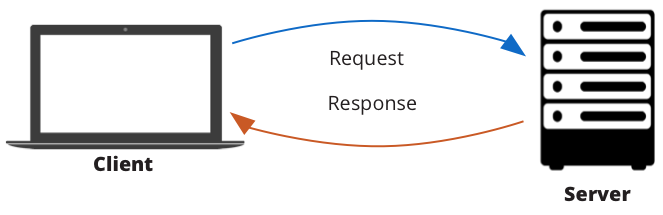
\includegraphics[height=3cm]{prosta_komunikacja2.png}
	\end{center}
\end{frame}

\begin{frame}{SignalR}
	\begin{center}
		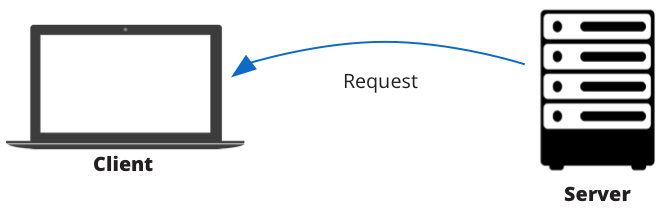
\includegraphics[height=3cm]{signalr1.png}
	\end{center}
\end{frame}

\begin{frame}{SignalR}
	\begin{center}
		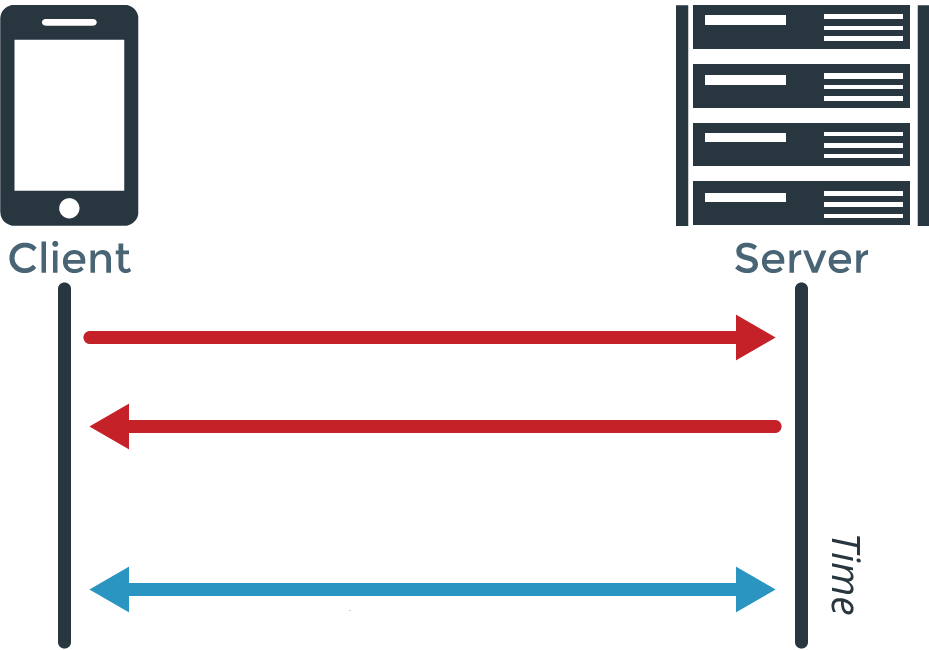
\includegraphics[height=5cm]{websocket1.png}
	\end{center}
\end{frame}

\begin{frame}{Nowe aplikacje}
	\begin{center}
		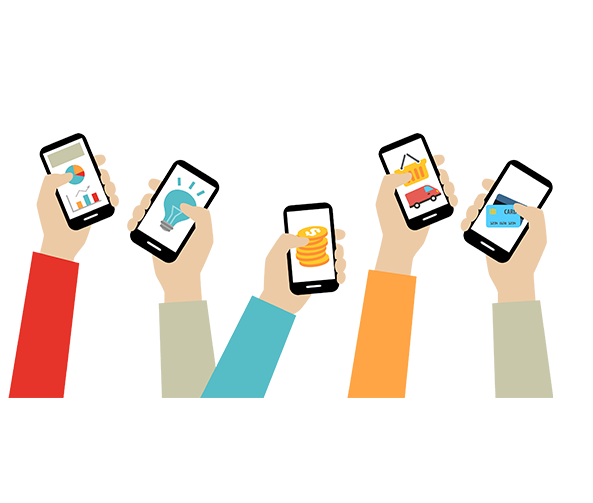
\includegraphics[height=5cm]{phone2.png}
	\end{center}
\end{frame}

\begin{frame}{}
	\begin{center}
		\Huge{To jeszcze nie koniec opowieści...}
	\end{center}
\end{frame}

\begin{frame}{}
	\begin{center}
		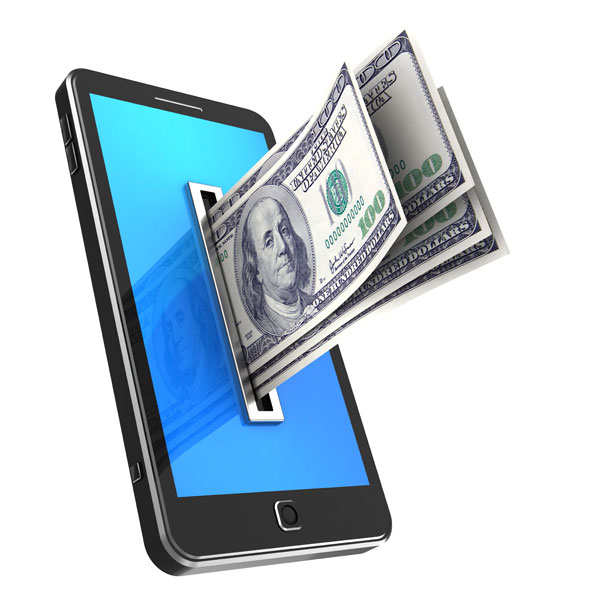
\includegraphics[height=5cm]{wallet1.jpg}
	\end{center}
\end{frame}

\begin{frame}{Wirtualne portfele}
	\begin{center}
		\begin{tabular}{ c c }
  			
\includegraphics[height=3cm]{wallet2.png} & 
\includegraphics[height=1.5cm]{prepaid1.png}
		\end{tabular}
	\end{center}
\end{frame}

\begin{frame}{Wirtualne portfele}
	\begin{huge}
		\begin{itemize}[<+->]
			\item Account
			\item Card
		\end{itemize}
	\end{huge}
\end{frame}

\begin{frame}{Komunikacja}
	\begin{huge}
		\begin{itemize}[<+->]
			\item Account -> Card
			\item Company -> Account
			\item Employee -> Account
		\end{itemize}
	\end{huge}
\end{frame}

\begin{frame}{}
	\begin{center}
		\Huge{Problemy}
	\end{center}
\end{frame}

\begin{frame}{Problemy}
	\begin{center}
		\Huge{Transakcyjność}
	\end{center}
\end{frame}

\begin{frame}{Komunikacja komponentów}
	\begin{center}
		\Huge{Kolejki}\\
		\huge{(Queue)}
	\end{center}
\end{frame}

\begin{frame}{}
	\begin{center}
		\Huge{<<Wyjaśnić czym są Queue>>}
	\end{center}
\end{frame}

\begin{frame}{}
	\begin{huge}
		\begin{itemize}[<+->]
			\item Company -> Account -> Card
			\item Employee -> Account -> Card
		\end{itemize}
	\end{huge}
\end{frame}

\begin{frame}{}
	\begin{huge}
		\begin{itemize}[<+->]
			\item Employee -> Restaurant -> Account -> Card
			\item Card -> Account
		\end{itemize}
	\end{huge}
\end{frame}


\begin{frame}{}
	\begin{center}
		\Huge{To póki co koniec opowieści}
	\end{center}
\end{frame}

\begin{frame}{}
	\begin{huge}
		\begin{itemize}[<+->]
			\item Aplikacje się rozbudowują
			\item Różne rodzaje komunikacji
		\end{itemize}
	\end{huge}
\end{frame}

\begin{frame}{}
	\begin{huge}
		\begin{itemize}[<+->]
			\item Fire-and-wait
			\item Fire-and-forget
			\item SignalR
			\item Kolejki
		\end{itemize}
	\end{huge}
\end{frame}

\begin{frame}{}
	\begin{center}
  		
\includegraphics[height=4cm]{ok.png} \\
		\Huge{Dziękuję!}
	\end{center}
\end{frame}


\end{document}